 \documentclass[a4paper,10pt]{article}
%DIF LATEXDIFF DIFFERENCE FILE
%DIF DEL ipfjes-interview.tex   Tue Jul 11 10:26:32 2017
%DIF ADD ../ipfjes-sop.tex      Tue Jul 11 09:06:04 2017
 
 %set font to Arial
 %\usepackage{fontspec}
 %\setmainfont{Arial}
 \usepackage{helvet}
 \renewcommand{\familydefault}{\sfdefault}
 
 %graphics
 \usepackage{graphicx}
 %\usepackage{subfigure}
 \usepackage{pslatex}
 \usepackage{pstricks}
 
 %math equations
 \usepackage{amsmath}
 
 %python code
 %\usepackage{minted}
 
 %headers
 \usepackage{fancyhdr}
 \pagestyle{fancy}
 \lhead{IRAS Project ID: 203355}
 \chead{}
%DIF 26c26
%DIF <  \rhead{clinicaltrials.gov reference}
%DIF -------
 \rhead{clinicaltrials.gov: NCT03211507} %DIF > 
%DIF -------
 \lfoot{IPF JES}
%DIF 28c28
%DIF <  \cfoot{Interview Schedule v0.4}
%DIF -------
 \cfoot{Standard Operating Procedure v0.5} %DIF > 
%DIF -------
 \rfoot{\today}
 
 
 %display URLS
 \usepackage{url}
 
 %hyperlinks
 \usepackage{hyperref}
 
 %comments
 \usepackage{verbatim}
 
 %nice tables
 \usepackage{booktabs}
 \newcommand{\ra}[1]{\renewcommand{\arraystretch}{#1}}
 
 %multi rows for the nice tables
 %\usepackage{multirow} 
 
 %nice diplay of code
 %\usepackage{minted}

%nice references
 \usepackage[super]{natbib}
 
 %some maths
 \usepackage{amsmath}
 
 %margins
 %\usepackage{geometry}
 %\geometry{verbose,a4paper,tmargin=60mm,bmargin=25mm,lmargin=25mm,rmargin=25mm}
 
 %in line citations
 %\usepackage{bibentry}
 
 %\hyphenpenalty=10000
 
 %\nobibliography*


%ability to continue an enumerated list
\usepackage{enumitem}

 
 
%DIF PREAMBLE EXTENSION ADDED BY LATEXDIFF
%DIF UNDERLINE PREAMBLE %DIF PREAMBLE
\RequirePackage[normalem]{ulem} %DIF PREAMBLE
\RequirePackage{color}\definecolor{RED}{rgb}{1,0,0}\definecolor{BLUE}{rgb}{0,0,1} %DIF PREAMBLE
\providecommand{\DIFaddtex}[1]{{\protect\color{blue}\uwave{#1}}} %DIF PREAMBLE
\providecommand{\DIFdeltex}[1]{{\protect\color{red}\sout{#1}}}                      %DIF PREAMBLE
%DIF SAFE PREAMBLE %DIF PREAMBLE
\providecommand{\DIFaddbegin}{} %DIF PREAMBLE
\providecommand{\DIFaddend}{} %DIF PREAMBLE
\providecommand{\DIFdelbegin}{} %DIF PREAMBLE
\providecommand{\DIFdelend}{} %DIF PREAMBLE
%DIF FLOATSAFE PREAMBLE %DIF PREAMBLE
\providecommand{\DIFaddFL}[1]{\DIFadd{#1}} %DIF PREAMBLE
\providecommand{\DIFdelFL}[1]{\DIFdel{#1}} %DIF PREAMBLE
\providecommand{\DIFaddbeginFL}{} %DIF PREAMBLE
\providecommand{\DIFaddendFL}{} %DIF PREAMBLE
\providecommand{\DIFdelbeginFL}{} %DIF PREAMBLE
\providecommand{\DIFdelendFL}{} %DIF PREAMBLE
%DIF END PREAMBLE EXTENSION ADDED BY LATEXDIFF
%DIF PREAMBLE EXTENSION ADDED BY LATEXDIFF
%DIF HYPERREF PREAMBLE %DIF PREAMBLE
\providecommand{\DIFadd}[1]{\texorpdfstring{\DIFaddtex{#1}}{#1}} %DIF PREAMBLE
\providecommand{\DIFdel}[1]{\texorpdfstring{\DIFdeltex{#1}}{}} %DIF PREAMBLE
%DIF END PREAMBLE EXTENSION ADDED BY LATEXDIFF

\begin{document}

 %\author{Carl Reynolds \\
 %\small National Heart \& Lung Institute, Imperial College London }

 %\pagenumbering{gobble}

 \pagestyle{fancy}

 %\pagestyle{empty}

% \maketitle


\section*{\DIFdelbegin \DIFdel{Interview Schedule }\DIFdelend \DIFaddbegin \DIFadd{Standard Operating Procedure }\DIFaddend for \DIFaddbegin \DIFadd{case and control recruitment and exposure assessment in }\DIFaddend the Idiopathic Pulmonary Fibrosis Job Exposure Study (IPF JES)}

\DIFaddbegin \tableofcontents

\section{\DIFadd{Scope and applicability}}

\DIFadd{The purpose of this SOP is to describe the instructions for the enrolment of cases and controls, exposure assessment, and genetic testing in the IPF JES.
}

\section{\DIFadd{Introduction}}

\DIFadd{The objective of IPF JES is to characterize and measure job exposures as an occupational determinant of Idiopathic Pulmonary Fibrosis (IPF). This will be achieved through a case-control study in which historic job exposures are measured using a validated semi-structured interview. A blood test will also be obtained to investigate interaction between job exposures and IPF genetic susceptibility factors.   
}

\section{\DIFadd{Recruitment}}

\subsection{\DIFadd{Recruitment of cases}}

\DIFadd{See figure ~\ref{fig:caserec}
}

\DIFadd{Cases will be recruited from male patients with a new diagnosis of IPF made during the study period within the research network.
}

\DIFadd{All clinic patients who meet the case inclusion criteria will be provided with a participant information sheet and participant job history sheet. Patients will be enrolled into the study, blood will be drawn, and a case-report form will be completed. The case-report form and blood samples will be placed into a pre-paid Royal Mail container and put in a postbox. Inclusion and exclusion criteria will be checked as part of enrolment. 
}

\DIFadd{The central research team will be updated monthly with details of the number of eligible patients attending clinic, the number of eligible patients approached to participate in the study, and the number of patients agreeing to participate in the study.
}

\DIFadd{Recruitment of cases from a centre stops when the agreed centre target is met or the agreed centre recruitment period ends.
}

%DIF > need to update figures
%DIF > need to update letter to non-resp cons
%DIF > check clinic

\begin{figure}
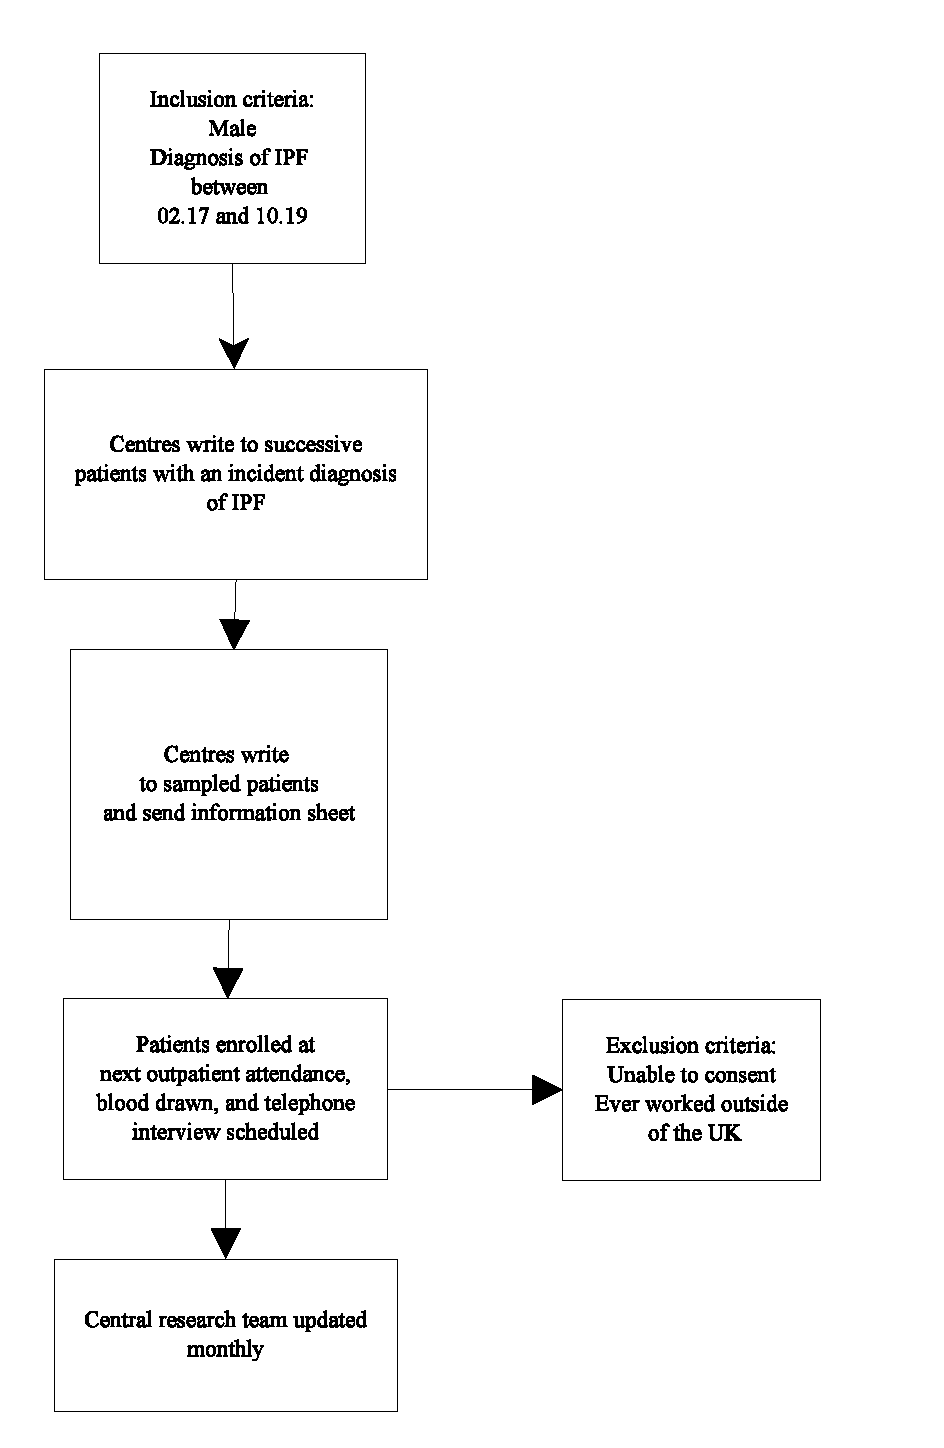
\includegraphics[scale=0.8]{fig/case-recruitment.eps}
\caption{\DIFaddFL{Case recruitment}\label{fig:caserec}}
\end{figure}
\subsection{\DIFadd{Recruitment of controls}}

\DIFadd{See figure ~\ref{fig:contrec}
}

 \DIFadd{Controls will be recruited from male patients with a new outpatient department attendance at the same hospital or trust that the cases originate from. Controls will be frequency matched on age to 5-year bands (e.g 50-54, 55-59, 60-64, 65-69, 70-74, 75-79, 80-84, 85+). The overall ratio of cases to controls will be 1:1.  
}

\DIFadd{A control clinic will be randomly selected (from all clinics, not limited to respiratory) at each centre. Paediatric clinics and gynaecological clinics will be excluded. This may be achieved by randomly sampling a list of all clinics, by randomly sampling a list of outpatient locations and a time of the week, or by other means. The central research team will provide support for this activity. 
}

\DIFadd{The local research team will write to the lead clinician for the selected clinic to obtain permission to recruit patients to the study. If permission is refused then the process is repeated until a lead clinician agrees. Once agreement is obtained this clinic will be the source clinic for all controls at that centre for the duration of the study.
 }

\DIFadd{Potential controls will be invited to participate in the study and provided with a patient information sheet when they attend the outpatient department. Patients will be enrolled into the study, blood will be drawn, the participant will be provided with a job history sheet, and a case-report form will be completed. The case-report form and blood samples will be placed into a pre-paid Royal Mail container and put in a postbox. Inclusion and exclusion criteria will be checked as part of enrolment.
}

\DIFadd{The central research team will be updated monthly with details of the number of eligible patients attending clinic, the number of eligible patients approached to participate in the study, and the number of patients agreeing to participate in the study.
}

\DIFadd{Recruitment of controls from a centre stops when recruitment of cases stops and one control for each case has been recruited or the agreed centre recruitment period ends.
}

\begin{figure}
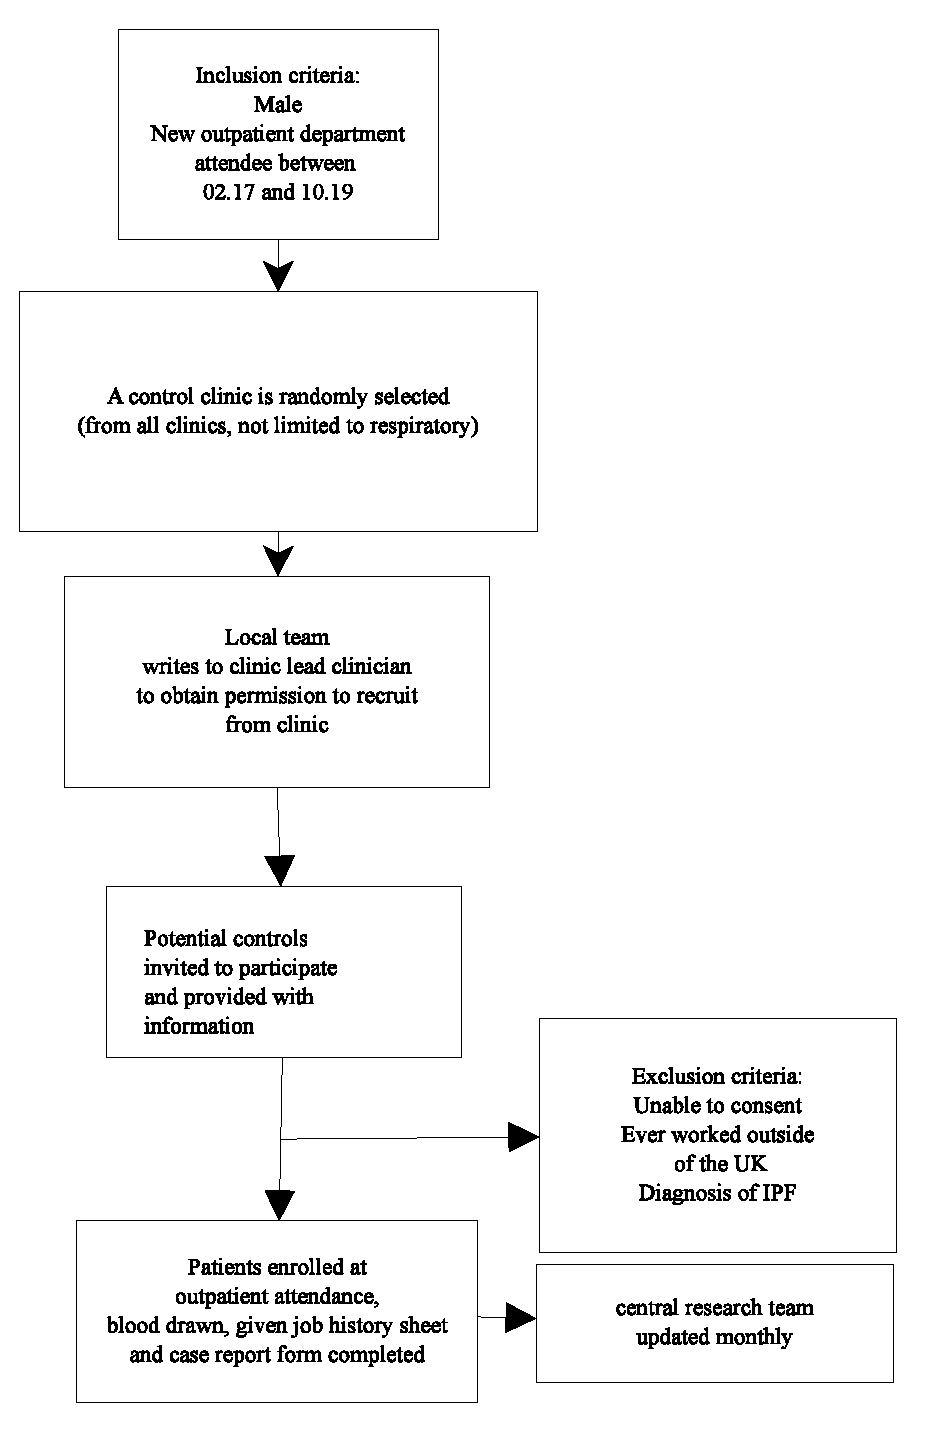
\includegraphics[scale=0.8]{fig/control-recruitment.eps}
\caption{\DIFaddFL{Control recruitment}\label{fig:contrec}}
\end{figure}

\section{\DIFadd{Exposure assessment}}

\DIFadd{The exposure assessment is carried out by the central research team by means of a computer-assisted telephone intereview.
}

\DIFaddend \section{Introduction}

Hello, my name is \textbf{name of researcher}. I am a doctor/nurse/research assistant calling as part of the IPF Job Exposure Study. Is this \textbf{name of participant}? 

I would like to ask you some questions about the jobs you have had, where you have lived, and \DIFdelbegin \DIFdel{your lifetime smokinghistory}\DIFdelend \DIFaddbegin \DIFadd{smoking}\DIFaddend . I would also like to record this call for our research if that's ok with you.  

Your answers will help us to understand the causes of IPF, make sure people get the right treatment, and ensure that controls of exposures at work are right so that we protect workers and prevent disease in the future.  

The interview should take about 30 minutes. Is now a good time to talk?

\section{Occupational \DIFdelbegin \DIFdel{and residential }\DIFdelend history} 

I want you to think about all of the jobs you've had. I know this can be hard, we'll try one at a time. 

Do you remember the first job that you had after school?

 \begin{enumerate} 
\item  What was the name of your job? \DIFaddbegin \DIFadd{(we record SOC2000 job title and map SOC90)
}\DIFaddend \item  What did you do in this job? \DIFaddbegin \DIFadd{(we record free text but also have a drop down of activities associated with asbestos exposure)
}\item  \DIFadd{What was the name of the company (if applicable)? (we record name and SIC code, we possibly link to open corporates company house record)
}\DIFaddend \item  What did the company make (if applicable)? \DIFaddbegin \DIFadd{(we record free text but also have a drop down of asbestos containing products)
}\item  \DIFadd{In what sort of working area did you spend most of your time? e.g Office, In the Open, Workshop, Construction Site, Factory (Light Industry), Heavy Industry (eg. Power Station), Hospital, School/University, Warehouse, “On Location”, various buildings, Shop, At Home, Ship/Ship yard, Other (specify) 
}\item  \DIFadd{Did you work full time? (if not specify average hours per week)
}\item  \DIFadd{Did you work all year round (if not specify months of the year)
}\DIFaddend \item  Do you remember how old you were or what year you started the job?
\item  Do you remember how old you were or what year you finished the job?
\item  Do you remember \DIFdelbegin \DIFdel{where you lived when you had that job?
}%DIFDELCMD < \item  %%%
\item%DIFAUXCMD
\DIFdel{Do you remember }\DIFdelend what job you had next?
 \end{enumerate} 

(1 through \DIFdelbegin \DIFdel{7 }\DIFdelend \DIFaddbegin \DIFadd{10 }\DIFaddend repeats until lifetime occupational history is complete. Standard occupational classification is used to code occupations)

\DIFdelbegin \DIFdel{`Trigger' }\DIFdelend \DIFaddbegin \DIFadd{Any reported contact with asbestos or `trigger' products (HSE list), industries (construction, factory work, power station work, other heavy industry, ships or ship yards), }\DIFaddend jobs (see Table ~\ref{table:top15pmr})\DIFdelbegin \DIFdel{prompt more detailed questioning regarding job process(es), materials used, and control measures (according to a validated structured subjective  assessment of past concentrations developed by John Cherrie) . Interviewers will receive training from John Cherrie on how to perform this assessment}\DIFdelend \DIFaddbegin \DIFadd{, and job processes prompts an asbestos exposure history (see later) to be taken}\DIFaddend .

\begin{table}
\begin{tabular}{llr}
\textbf{SOC90} &                                     \textbf{Occupation} &    \textbf{PMR} \\
\midrule
541 &                      Coach \& vehicle body builders &  528.18 \\
534 &          Metal plate workers, shipwrights, riveters &  416.64 \\
532 &         Plumbers, heating \& ventilating engineers  &  388.67 \\
570 &                               Carpenters \& joiners &  382.34 \\ 
896 &                  Construction \& related operatives &  359.23 \\
311 &                                 Building inspectors &  317.83 \\  
520 &           Production fitters (electical/electronic) &  300.15 \\
521 &        Electricians, electrical maintenance fitters &  264.12 \\
893 &  Electrical, energy, boiler \& related              &  252.09 \\
533 &                                 Sheet metal workers &  245.71 \\
301 &    Engineering technicians                          &  232.22 \\
506 &            Floorers, floor coverers, carpet fitters &  232.05 \\
913 &        Mates to metal/electrical \& related fitters &  230.89 \\
211 &                                Mechanical engineers &  217.44 \\
571 &                                      Cabinet makers &  215.36 \\ 
\bottomrule
\end{tabular}
\caption{Standard Occupational Classification 1990 code, Occupation, and Mesothelioma Proportional Mortality Ratio (PMR) for the top 15 significant (95\% CI does not include 100) PMRs. HSE data.}
\label{table:top15pmr}
\end{table}

\DIFaddbegin \newpage

\section{\DIFadd{Cohabitation history}}
\DIFaddend I'm going to ask you about \DIFdelbegin \DIFdel{places that you've lived }\DIFdelend \DIFaddbegin \DIFadd{people who have lived with you }\DIFaddend now. I\DIFdelbegin \DIFdel{know it might be difficult to remember, don't worry.
}\DIFdelend \DIFaddbegin \DIFadd{'m specifically interested in people that lived at home with you who went out to work.
}\DIFaddend 

\DIFdelbegin %DIFDELCMD < \begin{enumerate}[resume]
%DIFDELCMD < \item %%%
\DIFdel{What country were you born in? 
}%DIFDELCMD < \item %%%
\DIFdel{What place were you born in ?
}%DIFDELCMD < \item %%%
\DIFdel{Do you remember the places you lived when you were growing up? (until you finished school) 
}\DIFdelend \DIFaddbegin  \begin{enumerate} 
\DIFaddend \item When you were growing up \DIFdelbegin \DIFdel{who lived }\DIFdelend \DIFaddbegin \DIFadd{did anyone who went out to work live }\DIFaddend at home with you?
\item \DIFdelbegin \DIFdel{How long for}\DIFdelend \DIFaddbegin \DIFadd{What was the name of the person?
}\item \DIFadd{How long did they live with you}\DIFaddend ?
\item Do you remember what their job was?
 \end{enumerate} 


\section{Smoking history}

 \begin{enumerate} 
\item Have you ever smoked?
\item What old were you when you started smoking?
\item Do you still smoke?
\item How old were you, or when, did you stop smoking?
\item How many, on average, a day do you/did you smoke?
\item What do you/did you smoke?
 \end{enumerate} 

\section{mMRC dyspnoea questions} 

I would like to ask you some questions about being short of breath.

Are you:

 \begin{enumerate} 
\item Not troubled by breathless except on strenuous exercise?
\item Short of breath when hurrying on a level or when walking up a slight hill?
 \end{enumerate} 

Are you someone who:

 \begin{enumerate} [resume]
\item Walks slower than most people on the level, stops after a mile or so, or stops after 15 minutes walking at own pace?
\item Stops for breath after walking about 100 yds or after a few minutes on level ground?
 \end{enumerate} 

Are you:

 \begin{enumerate} [resume]
\item Too breathless to leave the house, or breathless when dressing/undressing?
 \end{enumerate} 

\section{Drug and medical history}

 \begin{enumerate} 
\item \DIFdelbegin \DIFdel{Do you take any regular medications ?
}%DIFDELCMD < \item %%%
\item%DIFAUXCMD
\DIFdel{What do you take these for?
}\DIFdelend \DIFaddbegin \DIFadd{Have you ever taken any heart medications such as amiodarone or flecainade, antibiotics such as nitrofurantoin, or immunosupressants and chemotherapy drugs such as, azathioprine, gefitinib, ifosfamide, melphalan, and rituximab? %DIF > http://www.pneumotox.com/pattern/view/224/XV.j/path-pulmonary-fibrosis-uip-pattern/
}\DIFaddend \item Do you have any other serious illnesses?
 \end{enumerate} 

\DIFaddbegin \section{\DIFadd{Family history}}

 \begin{enumerate} 
    \item \DIFadd{Does anyone in your family have scarring of their lungs (or pulmonary fibrosis)? 
}\item \DIFadd{If yes, who? 
} \end{enumerate} 

\section{\DIFadd{Asbestos exposure history}}

 \begin{enumerate} 
\item \DIFadd{Did you, or anyone close to you, ever work with or disturb material you suspected to be made from asbestos? This might include materials such as asbestos lagging, asbestos sprayed coatings, AIB(asbestos insulation board - e.g asbesolux, marinite, shipboard, LDR, turnasbestos etc) or corrugated roofing? (Yes, record what using free text, which job(s) associated with and John Cherrie item/No/Not known)
}\item \DIFadd{What was done with it? (free text and John Cherrie item)
}\item \DIFadd{How long did the task take and how often did you do it? (Record \% work time on task)
}\item \DIFadd{Where was the task completed? (free text and drop down e.g inside small room, inside large room, outside)
}\item \DIFadd{Did you wear a mask? (free text and drop down)
} \end{enumerate} 

\DIFaddend \section{(for cases only) how were you diagnosed}

 \begin{enumerate} 
    \item What took you to the doctor at the beginning of the illness? \DIFaddbegin \DIFadd{(e.g cough, breathlessness, incidental finding, other) 
} \end{enumerate} 

\section{\DIFadd{Ethnicity}}
\DIFadd{For the blood test that we have taken it would be helpful for us to know what ethnicity you are.
}

\DIFadd{To which of the following ethnic groups do you consider you belong?
}

 \begin{enumerate} 
\item \DIFadd{White
}\item \DIFadd{Black or Black British
}\item \DIFadd{Mixed
}\item \DIFadd{Chinese
}\item \DIFadd{Asian or Asian British
}\item \DIFadd{Other ethinic group (please specify)
}\DIFaddend  \end{enumerate} 
\DIFaddbegin 

\section{\DIFadd{Thank-you and updates}}
\DIFadd{Thank-you very much for participating today. Is there anything you'd like to ask us? Would you like to be kept updated on the study? How would you prefer to be updated? 
(Post or email, capture email if prefers email).
}

%DIF > think about crf

\section{\DIFadd{Venepuncture, sample storage, transportation, and processing}} 

\DIFadd{Venepuncture will be performed by a qualified practitioner. Sites will be provided with one 10ml EDTA tube and one 10ml SST tube per participant to obtain blood. Samples will be labelled with the participants unique research ID and posted using Royal Mail Safebox to a secure lab storage facility at NHLI where they will be kept in a -80 degree centigrade freezer. Royal Mail Safeboxes will be posted into a royal mail postbox by the local researcher; the hospital postal service will not
be used.
The sender will record the day of delivery and the research team will record receipt of the sample and keep an accurate record of its location. Analysis of samples will include DNA isolation and quantitative PCR taqman assay to investigate pre-defined SNPs of interest.
}

\section{\DIFadd{Unique research IDs}}

\DIFadd{Each participant will be assigned a unique research ID which will be used to label the Case Report Form and blood tubes. The ID will be 6 digits long. The first 2 digits will be the assigned centre ID. The subsequent 4 digits can be assigned to cases and controls as the centre wishes so long as there are no repeats.
}

\begin{table}[] %DIF >  http://www.tablesgenerator.com/latex_tables
    \centering
    \begin{tabular}{ll}
    \textbf{\DIFaddFL{Organisation}}                                           & \textbf{\DIFaddFL{Centre ID}} \\
        \midrule 
        \DIFaddFL{Heart of England NHS Foundation Trust                  }& \DIFaddFL{01        }\\
        \DIFaddFL{Morriston Hospital                                     }& \DIFaddFL{02        }\\
        \DIFaddFL{Nottingham University Hospitals NHS Trust              }& \DIFaddFL{03        }\\
        \DIFaddFL{Southampton University Hospitals NHS Trust             }& \DIFaddFL{04        }\\
        \DIFaddFL{University Hospital of South Manchester                }& \DIFaddFL{05        }\\
        \DIFaddFL{Papworth Hospital NHS Foundation Trust                 }& \DIFaddFL{06        }\\
        \DIFaddFL{Royal Devon and Exeter NHS Foundation Trust            }& \DIFaddFL{07        }\\
        \DIFaddFL{Aintree University Hospitals NHS Foundation Trust      }& \DIFaddFL{08        }\\
        \DIFaddFL{North Bristol NHS Trust                                }& \DIFaddFL{09        }\\
        \DIFaddFL{Imperial College Healthcare NHS Trust                  }& \DIFaddFL{10        }\\
        \DIFaddFL{Aberdeen Royal Infirmary                               }& \DIFaddFL{11        }\\
        \DIFaddFL{Glasgow Royal Infirmary                                }& \DIFaddFL{12        }\\
        \DIFaddFL{Royal Infirmary of Edinburgh                           }& \DIFaddFL{13        }\\
        \DIFaddFL{The Newcastle Upon Tyne Hospitals NHS Foundation Trust }& \DIFaddFL{14        }\\
        \DIFaddFL{Taunton and Somerset NHS Foundation Trust              }& \DIFaddFL{15        }\\
        \DIFaddFL{Leeds Teaching Hospitals NHS Trust                     }& \DIFaddFL{16        }\\ 
        \bottomrule 
    \end{tabular}
    \caption{\DIFaddFL{Centre study IDs}}

\end{table}

\section{\DIFadd{Study documentation and logs}}

\DIFadd{To meet GCP and HTA requirements the local team will maintain a local site study file. The local site file contains:
}

  \begin{enumerate} 
     \item \DIFadd{site delegation log (statement of activities document may be used)
     }\item \DIFadd{CVs and GCP certificates for research personnel listed in the delegation log
     }\item \DIFadd{study approvals
     }\item \DIFadd{study protocol 
     }\item \DIFadd{study standard operating procedure 
     }\item \DIFadd{study recruitment bundle (participant information sheet, consent form, job history sheet, case report form)
     }\item \DIFadd{study training log (ipfjes-tlog.docx)
     }\item \DIFadd{participation (screening) log (ipfjes-plog.xlsx)
     }\item \DIFadd{sample log (ipfjes-slog.xlsx)
     }\item \DIFadd{adverse event log (ipfjes-alog.xlsx)
     }\item \DIFadd{general notes (ipfjes-general-notes.docx)
     }\item \DIFadd{signed consent forms
 } \end{enumerate} 


\DIFadd{It is acceptable for some or all of these to be stored electronically. At the end of the study the central research team will be responsible for archiving local site files.
}


\section{\DIFadd{Tissue-tracking and communication}}

\DIFadd{The local team will track tissue obtained from research participants by emailing the central research team with the name and research ID of the research participant to inform them when samples are sent.
}\DIFaddend 

\end{document}

